\documentclass[fleqn,usenatbib]{mnras}

\usepackage{newtxtext,newtxmath}

%\usepackage{mathptmx}
%\usepackage{txfonts}

\usepackage[T1]{fontenc}
\usepackage{ae,aecompl}

\usepackage{graphicx}	% Including figure files
\usepackage{amsmath}	% Advanced maths commands
\usepackage{amssymb}	% Extra maths symbols

%%%%%%%%%%%%%%%%%%%%%%%%%%%%%%%%%%%%%%%%%%%%%%%%%%%%%%%%%%%%

\title{Instrumental Calibration Requirements}

% The list of authors, and the short list which is used in the headers.
% If you need two or more lines of authors, add an extra line using \newauthor
\author[Kumar et al.]{Jais Kumar,$^{1}$\thanks{E-mail: jaisk.rs.phy16@iitbhu.ac.in}
Prasun Dutta,$^{1}$
Third Author$^{2,3}$
and Fourth Author$^{3}$
\\
% List of institutions
$^{1}$Department of Physics, Indian Institute of Technology (Banaras Hindu University), Varanasi - 221005, India\\
$^{2}$Address two\\
$^{3}$Another Department, Different Institution, Street Address, City Postal Code, Country
}
\date{Accepted XXX. Received YYY; in original form ZZZ}
\pubyear{2019}

% Don't change these lines
\begin{document}
\label{firstpage}
\pagerange{\pageref{firstpage}--\pageref{lastpage}}
\maketitle

\section{Abstract}

\section{Introduction}

\section{Analytical Calculation}
\subsection{Visibility}
Each antenna of a radio interferometer records the electric fields incident on its cross dipoles modified by the complex gain arising from the entire electronic chain. In addition to the electronic chain, the ionosphere also adds to the complex gain. The interferometers evaluate the spatial coherence function of the source or the visibility as a function of the inverse angular scale in the sky or baseline.  The visibilities are calculated by doing cross correlating the electric fields from each pair of antenna using digital correlates. A pair of antenna measure the value of the visibility function at a baseline given by their positional separation projected perpendicular to the direction of observation in units of observing wavelengths. The correlations are performed for a certain integration time such that the visibilities hence calculated are not affected by the time-width smearing. In this work, we consider all effects in a single frequency channel and hence we will not explicitly write the frequency dependence. While doing the data analysis, with help of primary calibrators and self calibration method the antenna gains are calculated as a function of time and the visibilities are calibrated for the complex gains and prepared for further analysis. Note that the gain calibration can be only done to certain accuracy depending on the quality of the primary calibrators, receiver noise, ionospheric stability etc. We shall refer to the uncalibrated part of the gain as residual gain.

If a high dynamic range observation is required to resolve the science questions, the residual gains need to be minimised to a certain accuracy. In this work, we access the effect of the residual gain in the visibility prepared for the science analysis. The residual complex gain from antenna A can be modelled as 
\begin{equation}
 g_A(t) = \left [ 1+\delta_A(t) \right ]e^{i\phi_A(t)},
\end{equation}
where both $\delta_A$ and $\phi_A$ are much smaller than unity and randomly distributed. 
Hence, the visibility $V_{AB}^M(t)$ measured by antenna pair A and B in presence of the residual gain can be written in terms of  the visibility function from the sky $V_{AB}^S = < E^*_A E_B>$  as
\begin{equation}
    V_{AB}^M(t) = < \left [ 1+\delta_A(t) \right ] \left [1+\delta_B(t)\right ] e^{i(\phi_B(t)-\phi_A(t))}> V_{AB}^S,
\end{equation}
note that a primary assumption in radio interferometry is that the specific intensity and hence the visibility function of the source is independent of time (reference synthesis imaging).  Clearly, the excess or the residual visibility recorded by the interferometer due to the residual gain error can be written as
\begin{equation}
    V_{AB}^R (t)= V_{AB}^M(t) - V_{AB}^S.
\end{equation}
It is required to estimate  the residual visibilities in case of a high dynamic range observations. If we assume that $
V_{AB}^S = V_{AB}^{S, H} + V_{AB}^{S, L} $, where $\mid V_{AB}^{S, H} \mid >> \mid V_{AB}^{S, L} \mid $, then retrive the $V_{AB}^{S, L} $ signal from the observed visibilities it is required that $\mid V_{AB}^R (t) \mid < V_{AB}^{S, L} $. 

The statistical nature of the signal is often extracted from the power spectrum of the sky brightness distribution. Bharadwaj and Sethi .. have showed that the power spectrum of the sky brightness distribution at a given baseline can be directly estimated by correlating the visibilities at the same baseline . In eqn~(2), we have neglected the receiver noise. In most of the radio interferometric observations the receiver noise present at a given baseline supersedes the sky visibility at that baseline. Cite has proposed a visibility based the power spectrum estimator, where instead of correlating the visibilities in the same baselines, visibility correlation at nearby baselines are used, that is 
\begin{equation}
    \mathcal{E} [P(U)]  = \langle \mid V(\vec{U})^* V(\vec{U}+\Delta \vec{U}) \mid \rangle.
\end{equation}
This estimator assumes that the noise  is not correlated between any other baseline, however, the visibility function of the source is correlated in the nearby baselines. In this work we shall investigate the validity of this assumption. 

\subsection{Modelling the gain errors}
We assume that the quantities $\delta_A(t)$ and $\phi_A(t)$ that characterises the residual gain error  quantities follow Gaussian distribution with mean zero. It has been observed that there exists non-zero time correlation in the residual gains. We quantify this time correlation using a two point correlation function as 

\begin{eqnarray}
\xi_{A}(\tau) &=& \langle \delta_A(t) \delta_A(t+\tau)\rangle,\ \ \ \ \ \ \ \  \sigma_{\delta}^2 =  \xi_A(0) =  \langle \delta_A^2 \rangle \\ \nonumber
\Phi_{A}(\tau) &=& \langle \phi_A(t) \phi_A(t+\tau)\rangle,\ \ \ \ \ \ \ \  \sigma_{\phi}^2 =  \xi_A(0) =  \langle \phi_A^2 \rangle.
\end{eqnarray}
Here  eg, $\xi_A (t) = 0\  \forall\  \tau \neq 0$ corresponds to the case of no time correlation. Here we assume that residual gain errors from different antennae are not correlated and  there is no correlation between the amplitude and the phase gain errors of any  antenna. 


======================


We assume that 
Visibility is defined as the correlation of the output signal from two different antenna. The radio antenna measures the electric field signal coming from the sky. Let's say the sky signal is $E_A$ and $E_B$ for antenna A and B respectively. The measured electric field differs from the true sky electric field because of instrumental response and atmospheric effects which is collectively known as the gain of the antenna. This gain is in general a time dependent complex quantity. The quantity visibility which is the correlation of output electric field coming from antenna pair A, B can be given as:
\begin{equation}
    V_{AB}^O = <g^*_A(t)g_B(t)> < E^*_A(t)E_B(t)>
\end{equation}
where 
\begin{equation}
    \begin{split}
     g_A(t) = (1+\delta_A(t))e^{i\phi_A(t)} \\ g_B(t) = (1+\delta_B(t))e^{i\phi_B(t)}   
    \end{split}
\end{equation}
 are the antenna based complex gains and * denotes the complex conjugate, here $\delta's$ and $\phi's$ are respectively the residual amplitude and phase gain errors of the different antennae and subscripts denotes antenna.\\
Observed visibility can be written as
\begin{equation}
\begin{split}
    V_{AB}^O(t) = <(1+\delta_A(t))(1+\delta_B(t))e^{i(\phi_B(t)-\phi_A(t))}> \\ < E^*_A(t)E_B(t)>
\end{split}
\end{equation}
If we know the source positions exactly (like for case of point source sky) we can subtract the true sky visibility $V_{AB}^S(t) = <E^*_A(t)E_B(t)> $ from the observed visibility.After doing so we get the residual visibility $V^R_{AB}(t)$
\begin{equation}
    V_{AB}^R (t)= V_{AB}^O(t) - V_{AB}^S(t)
\end{equation}
where $V_{AB}^S(t) =<E^*_A(t)E_B(t)> $ is the sky visibility.\\
\textbf{Residual Gain Model}
Residual gain errors $\delta_A$ \& $\phi_A$ are chosen from Gaussian distribution with following properties
 \begin{equation}
 \begin{split}
     <\delta_A(t) = 0>\\<\delta_A(t) \delta_A(t+\tau)> = \xi_A(\tau)\\\xi_A(0) = <\delta^2_A(t)> = \sigma^2_{\delta}
 \end{split}
 \end{equation}
 Similarly for residual phase gain error $ \phi $\\
 Here we assume that residual gain errors from different antennae are not correlated, also there is no correlation between amplitude and phase gain errors of an antenna, we also ignore any third or higher order terms in residual gain errors.\\
 \textbf{Delta variance}
\begin{equation}
    \Delta(\Gamma) = \frac{1}{\Gamma} \int _0 ^{\Gamma} \xi (t) dt
\end{equation}
where $\Gamma = (\frac{2\Delta U T_{24}}{2\pi U})$ is the visibility correlation length within which we are correlating the visibilities to calculate the power spectrum.\\
We modelled the residual gain errors as time correlated Gaussian random variables where the correlation function is given using power law. To generate residual gain errors we use the power spectrum of the form
\begin{equation}
    P(\omega) = \omega ^{-\alpha}
\end{equation}
which gives the correlation function of the form
\begin{equation}
    \xi(\tau) = A\tau^{-(1-\alpha)}
\end{equation}
The delta variance of this correlation function will be
\begin{equation}
     \Delta(U) = \Delta_0 U^{1-\alpha}
\end{equation}
 $\Delta_0 = \frac{A}{\alpha} (\frac{\Delta U T_{24}}{\pi})^{-(1-\alpha)}$, here $T_{24}$ is the 24 hour time in seconds. 
 we assume that the delta variance of amplitude gain errors for different antenna are same, similarly for phase gain errors.\\
\subsection{Residual Power spectrum}
The power spectrum is the correlation of the two visibility at baselines U and $U+\Delta U$ as
\begin{equation}
    P(U) = <V(U)^* V(U+\Delta U)>
\end{equation}
Residual power spectrum is calculated using the binned power spectrum estimator. In which we correlate all the visibility points falling within a circle of radius $\Delta U$  centered at baseline U. From the residual visibility we calculated the residual power spectrum.  As we correlate the visibilities within some range $\Delta U$ at baseline U we can replace the correlation term in residual power spectrum by $\Delta(\Gamma)$, here $\Gamma$, the visibility correlation length is function of U and $\Delta U$ .\\
Given the baseline configuration there will be various type of baseline pairs which will measure the visibility at various points in uv space. Observe visibility apart from signal and foreground have one more component which is thermal noise. Thermal noise is assumed to be Gaussian uncorrelated variable which means that the noise in the two different baselines or the noise in the visibility coming from the same baseline pair but measured at different time will be uncorrelated. To remove this thermal noise bias we didn't consider the correlation of the visibility coming from the same antenna pair measured at same time.\\
Given a baseline configuration there will be many visibilities and hence various types of visibility pairs will be possible. We divide them in following three types\\
\begin{figure}
    \centering
    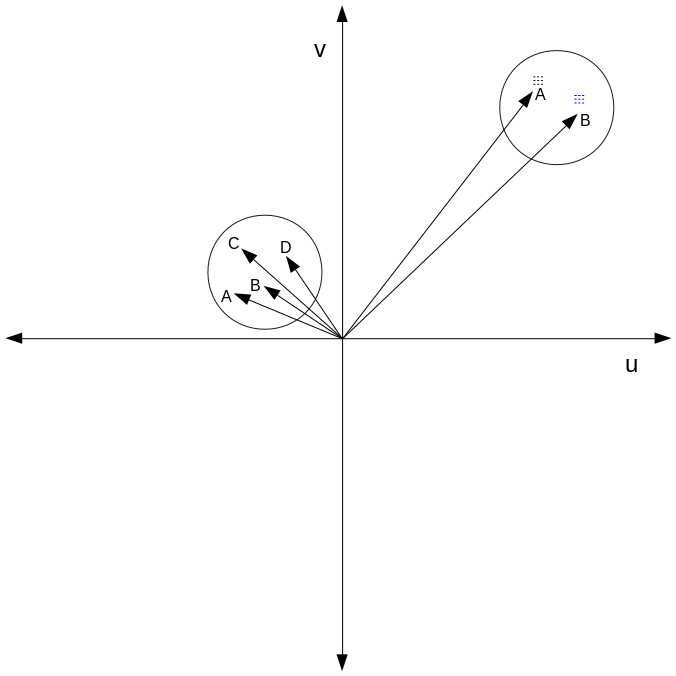
\includegraphics[width=0.5\textwidth]{Baseline_ABCD.png}
    \caption{This cartoon shows that at smaller baselines there will be more visibility points formed with different  antenna pairs while at larger baselines visibility points will be coming from same antenna pairs  }
    \label{fig:my_label}
\end{figure}
\textbf{CASE I:} {Visibility pairs of type $V_{AB}|V_{AB}$} \\
Here we consider the correlation of visibility pairs which are coming from the same antenna pairs say AB. In this case we consider only the visibility pairs which will be measured from the same antenna pair but at different time say one at time t and another at t'. In this case the residual power spectrum will be

\begin{equation}
    P_1^R(U) = [\xi_A(\tau) + \xi_B(\tau) + \chi_A(\tau) +\chi_B(\tau) ]P^S(U)
\end{equation}
where $\chi(\tau)$ is correlation of residual phase gain error. Subscripts A,B,C,D denotes the antenna.
Writing the correlation terms in terms of $\Gamma$
\begin{equation}
      P_1^R(U) = [2\Delta^{\delta}_0 U^{1-\alpha_{\delta}}+ 2\Delta^{\phi}_0 U^{1-\alpha_{\phi}}]P^S(U)
 \end{equation}
\textbf{CASE II:}{Visibility pairs of type $V_{AB}|V_{AC}$}\\
Another type of visibility pairs which will give the power spectrum is possible in which three antennae are involved. One pair coming from antenna AB and another say AC. Both pairs have one antenna in common.\\
(a) When measured at the same time this baseline pair will give the residual power spectrum

\begin{equation}
    P_2^R(U) = [\sigma^2_{\delta} + \sigma^2_{\phi}]P^S(U)
\end{equation}

(b) When the visibility from the two baseline pairs AB and AC are measured at different time in this case the residual power spectrum will be

\begin{equation}
    P_3^R(U) = [\xi_A({\tau}) + \chi_A(\tau)]P^S(U)
\end{equation}
or
\begin{equation}
      P_3^R(U) = [\Delta^{\delta}_0  U^{1-\alpha_{\delta}}+ \Delta^{\phi}_0 U^{1-\alpha_{\phi}}]P^S(U)
 \end{equation}
\textbf{CASE III:}{Visibility pairs of type $V_{AB}|V_{CD}$}\\
One possibility of visibility pair is this in which two visibilities are coming from the four different antennae .We consider here only those baseline pairs which are formed from 4 different antennae, lying within $\Delta U$ range at U. In this case the residual power spectrum will be
\begin{equation}
    P_4^R(U) = <V^R_{AB}(t)^* V^R_{CD}(t)>
\end{equation}
Using the properties of the residual gain errors we find that
\begin{equation}
    P_4^R(U) = 0
\end{equation}
Given the baseline configuration in total no of baselines lets assume $n_1$, is the no of baselines discussed in case I, $n_2$ is no of baselines discussed in case II and $n_3$ is no of baselines discussed in case II(a) and $n_4$ is no of baselines discussed in case III(b).
\begin{equation}
    n = n_1 + n_2 + n_3 + n_4
\end{equation}
The cartoon in figure 1 emphasizes the fact that there will be more antenna pairs at shorter separation and hence the lower baselines will be dominated by the visibility points of type II and III while at larger baselines we will have mostly those visibility points of type I which are formed from the same antenna pairs.\\

The total residual power spectrum in presence of the residual gain errors as modelled above will be sum of the residual power spectrum in the three cases discussed above.
So in the total residual power spectrum weightage of residual power spectrum from different cases will be different.
\begin{equation}
    P^R(U) =  \frac{n_1}{n} P_1^R(U) + \frac{n_2}{n} P_2^R(U) + \frac{n_3}{n} P_3^R(U) )
\end{equation}
as $P_4^R(U)$ is zero.\\
For a given baseline configuration to calculate the total residual power spectrum we consider two scenarios.\\
\textbf{Scene 1:}$n_1 = n_2 = n_3 = n_4 = \frac{n}{4}$ i.e. all the different correlation types have same contribution in total residual power spectrum.\\
Using the same power law index for residual amplitude and phase gain error i.e $\alpha_{\delta} = \alpha_{\phi} = \alpha$ and for fix $\Delta U$ we get
\begin{equation}
    {P^R(U)} = [\frac{3}{4}C_0U^{1-\alpha} + \frac{1}{4}C_1]{P^S(U)}
\end{equation}
Where constants $C_1$ and $C_2$ can be calculated using the parameters used. $\alpha = 0.03$ $\Delta U = 0.005 k\lambda$, $\sigma_{\delta}$ and $\sigma_{\phi}$. For $\sigma_{\delta} = 0.01\%$ and $\sigma_{\phi} = 0.01^{\circ}$, $C_0 = 2.27389\times 10^{-8}$  and $C_1 = 4.046\times10^{-8}$\\

\textbf{Scene 2: More Realistic Scenario:}\\
As for any given realistic baseline configuration the visibility points distribution in space highly depends on the baseline length U. Here we consider the fraction of various visibility pairs to be U dependent i.e. $n_1(U)$, $n_2(U)$, $n_3(U)$, $n_4(U)$. In this case we get
\begin{equation}
    {P^R(U)} = [C_0 \frac{2 n_1(U)+n_3(U)}{n}U^{1-\alpha} + C_1 \frac{n_2(U)}{n}]{P^S(U)}
    \end{equation}
We can model $\frac{n_1(U)}{n}$, $\frac{n_2(U)}{n}$, $\frac{n_3(U)}{n}$ as $A_1U^{a_1}$, $A_2U^{a_2}$, $A_3U^{a_3}$ respectively.
In figure 2 we plot the normalized residual power spectrum with baseline length for different set of values of A's and a's. 
a.) $A_1 = A_2 = A_3 = 0.25$, $a_1 = a_2 = a_3 = -0.25$\\
b.) $A_1 = 0.3, A_2 = 0.2, A_3 = 0.25$, $a_1 = -0.4, a_2 = -0.2, a_3 = -0.3$\\
c.) $A_1 = 0.3, A_2 = 0.1, A_3 = 0.25$, $a_1 = -0.5, a_2 = -0.3, a_3 = -0.25$\\

 We see that normalized residual power spectrum increases at larger baselines. This variation is different in different cases of type of baselines pairs. 
\begin{figure}
    \centering
    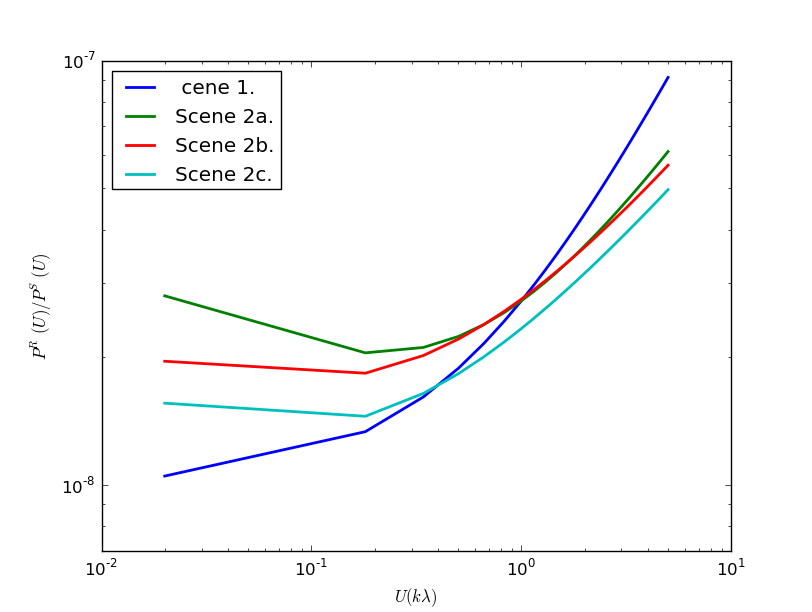
\includegraphics[width=0.5\textwidth]{ResPow_vsU_Nu.png}
    \caption{In this figure we have shown the variation of normalized residual power spectrum coming from the analytical calculations. We see that normalized residual power spectrum increases at larger baselines. This variation is different in different cases of type of baselines pairs. }
    \label{fig:Figure 3}
\end{figure}

\section{Simulation Results}
We consider only the extra-galactic point source component as our foreground model. To generate the realistic point source sky we use the differential source count relation from Intema et al. 2017, based on the TIFR GMRT SKY SURVEY at 150 MHz.
\begin{figure}
    \centering
    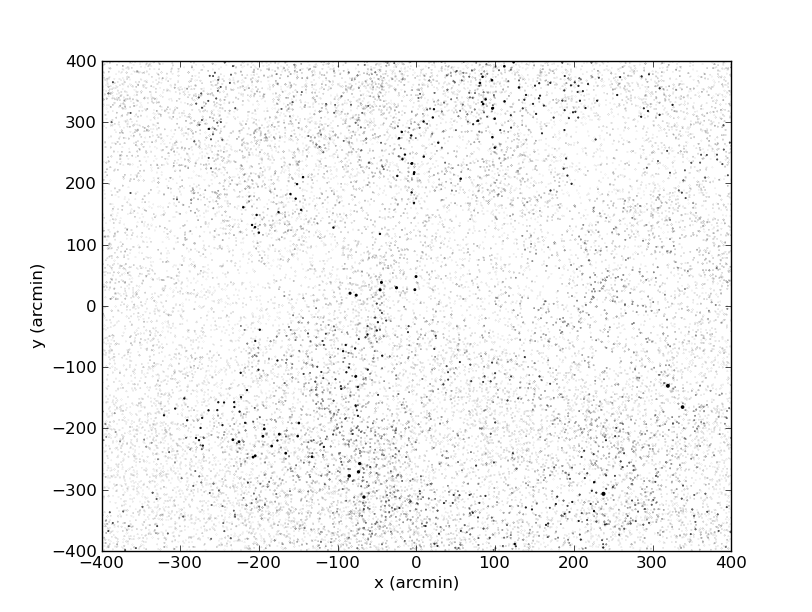
\includegraphics[width=0.5\textwidth]{cluster_sky.png}
    \caption{The point source foreground. x and y are the x positions and y positions of the sources from the pointing center in arc min.}
    \label{fig:my_label}
\end{figure}

\begin{equation}
log_{10}(S^{5/2}dN/dS)  = C_0 + \sum _{i=1}^{5}C_i\times[log_{10}(S)]^i
\end{equation}
where $C_i's$ are constants (values given in the reference paper). \\
We also consider the clustering of the point sources and include the clustering behaviour in our sky model. For this we use the results given in Rana and Bagla 2019. They used the TGSS - ADR1 data to study the clustering behaviour of point sources at 150 MHz.\\
In Figure 3 we show the simulated sky image. The radius of field of view of our sky was 400 arc min which contains around 20000 sources in the flux density ranging from 3 mJy to 100 Jy.
First we simulate the above sky model and estimated the model sky visibility then we simulated the residual gain errors based on the above discussed gain error model with the above foreground sky for full synthesis GMRT baseline configuration (total 8 hours of observation time) to estimate the true visibility. The frequency of observation was 130 MHz. Due to the computational limitations we consider only the single channel observation with channel width of 62.5 kHz. We subtract the model sky visibility from the true visibility which we call as residual visibility and then from the residual visibility we calculate the residual power. To see the statistics of residual power spectrum we consider the 128 realizations of such residual gain errors. finally we compare the residual power spectrum with the theoretical EoR power spectrum taken from Bharadwaj and Ali 2004.\\
\begin{figure}
    \centering
    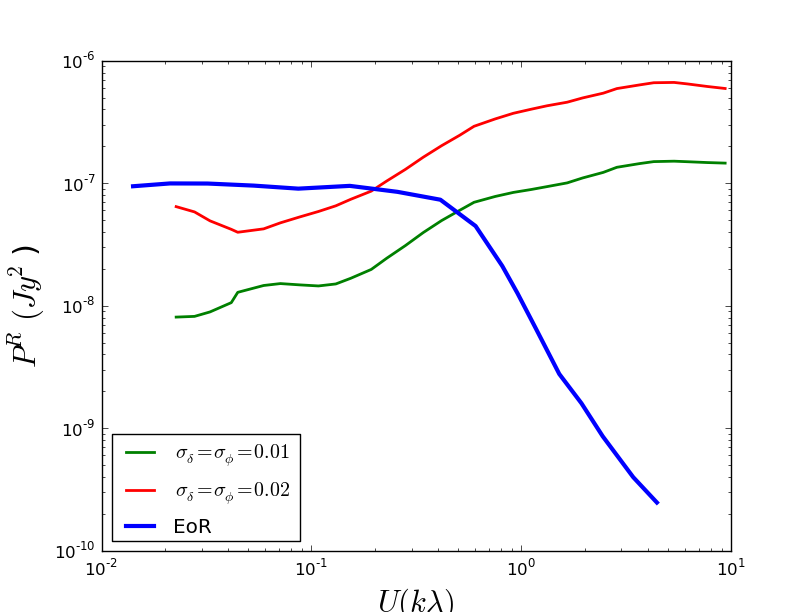
\includegraphics[width=0.5\textwidth]{ResPow_AP.png}
    \caption{Residual power spectrum plotted with baseline U. $\sigma_{\delta}$ is in percentage and $\sigma_{\phi}$ is in degree. we have applied the Gaussian smoothing with $\sigma = 2$ on the residual power spectrum.}
    \label{fig:my_label}
\end{figure}
\begin{figure}
    \centering
    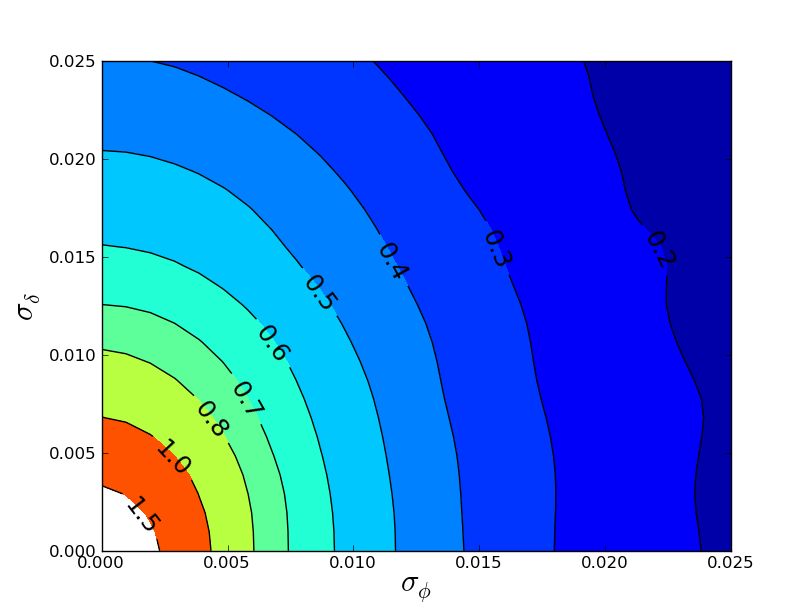
\includegraphics[width=0.5\textwidth]{SigDelvsSigPhi_Ucolor.png}
    \caption{This color plot showing the variation of $U_max$ as a function of residual amplitude and phase gain errors. The maximum allowed baseline length $U_max$ values are written over contour plots. Here amplitude gain errors $\sigma_{\delta}$ is in percent and $\sigma_{\phi}$ is in degree.}
    \label{fig:my_label}
\end{figure}
The power spectrum we used to generate the time correlated residual amplitude and phase gain errors is 
\begin{equation}
    P(\omega) = \omega ^{-\alpha}
\end{equation}
We choose value of $\alpha = 0.03$ and varied residual amplitude and phase gain errors from $0.01 \% - 0.03 \%$ and $0.01^{\circ} - 0.03^{\circ}$ to calculate the residual power spectrum. We use Gaussian smoothing function to smooth the residual power spectrum and finally compared it with theoretical EoR power spectrum. In Figure 4. what we have shown is the maximum allowed baseline length up to which EoR power spectrum can be recovered $U_{max}$. $U_{max}$ is the point where residual power spectrum crosses and exceeds the EoR power spectrum afterwards. \\
Also for fixed amount of residual amplitude and phase gain error we changed the slope $\alpha$ of the power spectrum (in equation 23) to see the effect of correlation on residual power spectrum. We varied $\alpha$ from 0.03 to 0.10 for both amplitude and phase and calculated the residual power spectrum and again from that by comparing with EoR power spectrum we find the $U_{max}$. In Figure 5. we show the variation of $U_{max}$ with varying correlation parameter. We find that as $\alpha$ becomes more and more negative the amplitude of residual power spectrum increases and hence the maximum allowed baseline length to recover the EoR signal decreases.

\begin{figure}
    \centering
    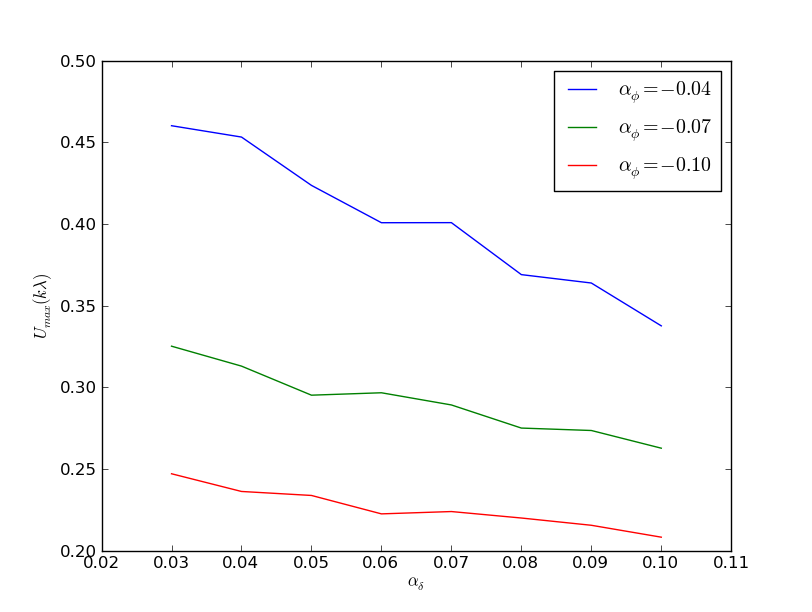
\includegraphics[width=0.5\textwidth]{Umax_AlpDel.png}
    \caption{Variation of $U_max$ as function of correlation parameter for residual amplitude gain error $\alpha_{\delta}$. Here we see that $U_{max}$ decreases with increasing $\alpha$ values.}
    \label{fig:my_label}
\end{figure}
\begin{figure}
    \centering
    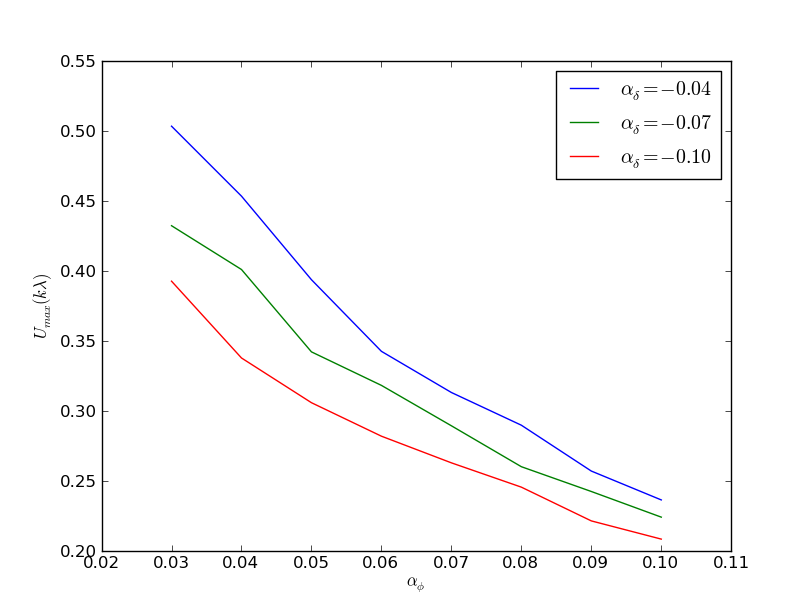
\includegraphics[width=0.5\textwidth]{Umax_AlpPhi.png}
    \caption{Variation of $U_max$ as function of correlation parameter for residual phase gain error $\alpha_{\phi}$. Here we also $U_{max}$ decreases with increasing $\alpha$ values.}  \label{fig:my_label}
\end{figure}

\section{Discussion and Conclusion}
The strong foreground in low frequency regime poses a huge challenge in observation of cosmological 21 cm signal. Foreground subtraction is essential in order to get the 21 cm signal from interferometric observations.
We have studied the point source foreground subtraction requirements in order to achieve the cosmological 21 cm signal in presence of residual gain errors. We have modeled the residual gain errors as time correlated Gaussian random variable which is more likely to be the case for an existing radio interferometer. We did the analytical calculations and later performed the simulations using GMRT baseline configuration at desired frequencies. Our results shows that for GMRT like array in order to achieve the residual signal bellow the cosmological 21 cm signal after subtracting the point source component of foreground the instrumental accuracy in amplitude and phase gain should be less than 0.02 percent and 0.02 degree respectively. For this much accuracy the allowed baseline range to recover the cosmological 21 cm signal is around 0.5 $k\lambda$. We took the correlation parameter 0.03 for both residual amplitude and phase gain errors in our detailed study. We also checked the correlation parameter dependency of the allowed baseline range, we found that as the gain errors will be more correlated residual signal will be stronger and allowed baseline range will be smaller. 
\end{document}
